\documentclass{article}
\usepackage[left=1in,top=0cm,right=1in,nohead,nofoot]{geometry} 
\usepackage{graphicx}

\begin{document}

\begin{figure}
\centering
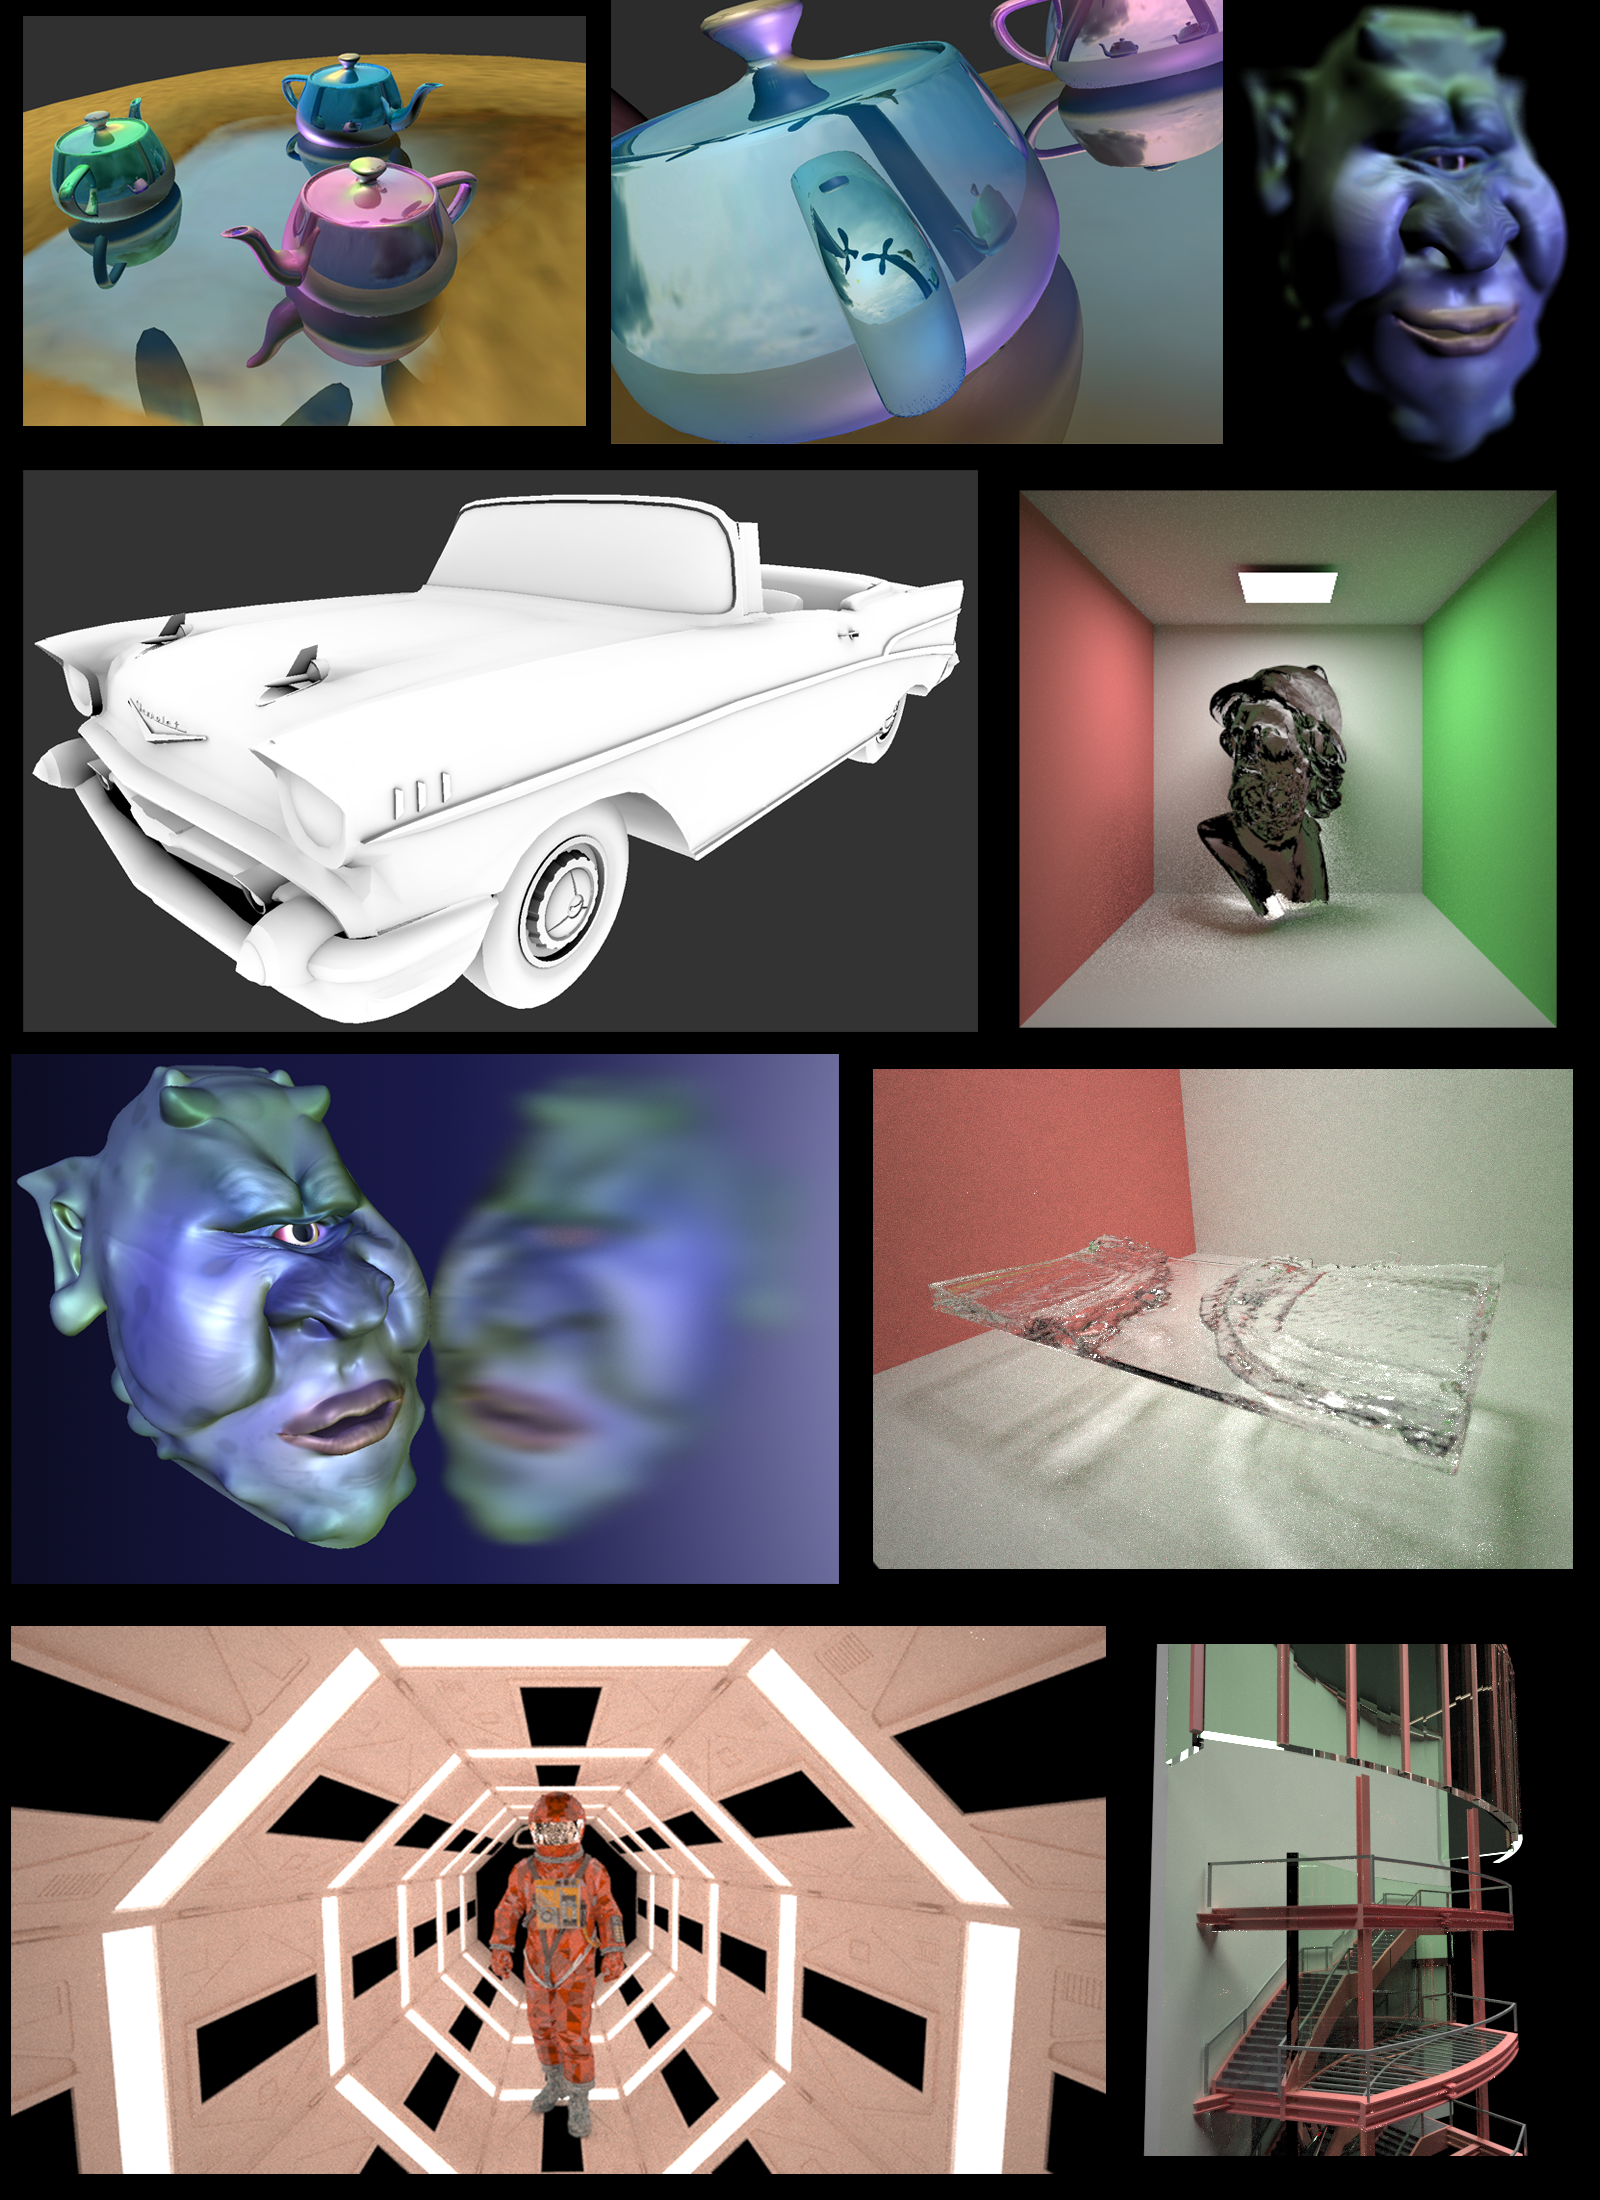
\includegraphics[width=6.5in]{images/composite.png}
\caption{\textbf{Selected Images.} \textbf{Top}: Interactive GPU ray tracing of dynamic objects.
        \textbf{Upper middle}: Interactive ambient occlusion and unbiased light transport on the GPU.
        \textbf{Lower Middle}: Glossy reflections on the GPU and caustics synthesized with Metropolis light transport.
        \textbf{Bottom}: Noise-aware Metropolis light transport.}
\end{figure}

\end{document}

